\section{DQN Algorithm}

\begin{frame}{DQN Algorithm}
    \begin{figure}
        \centering
        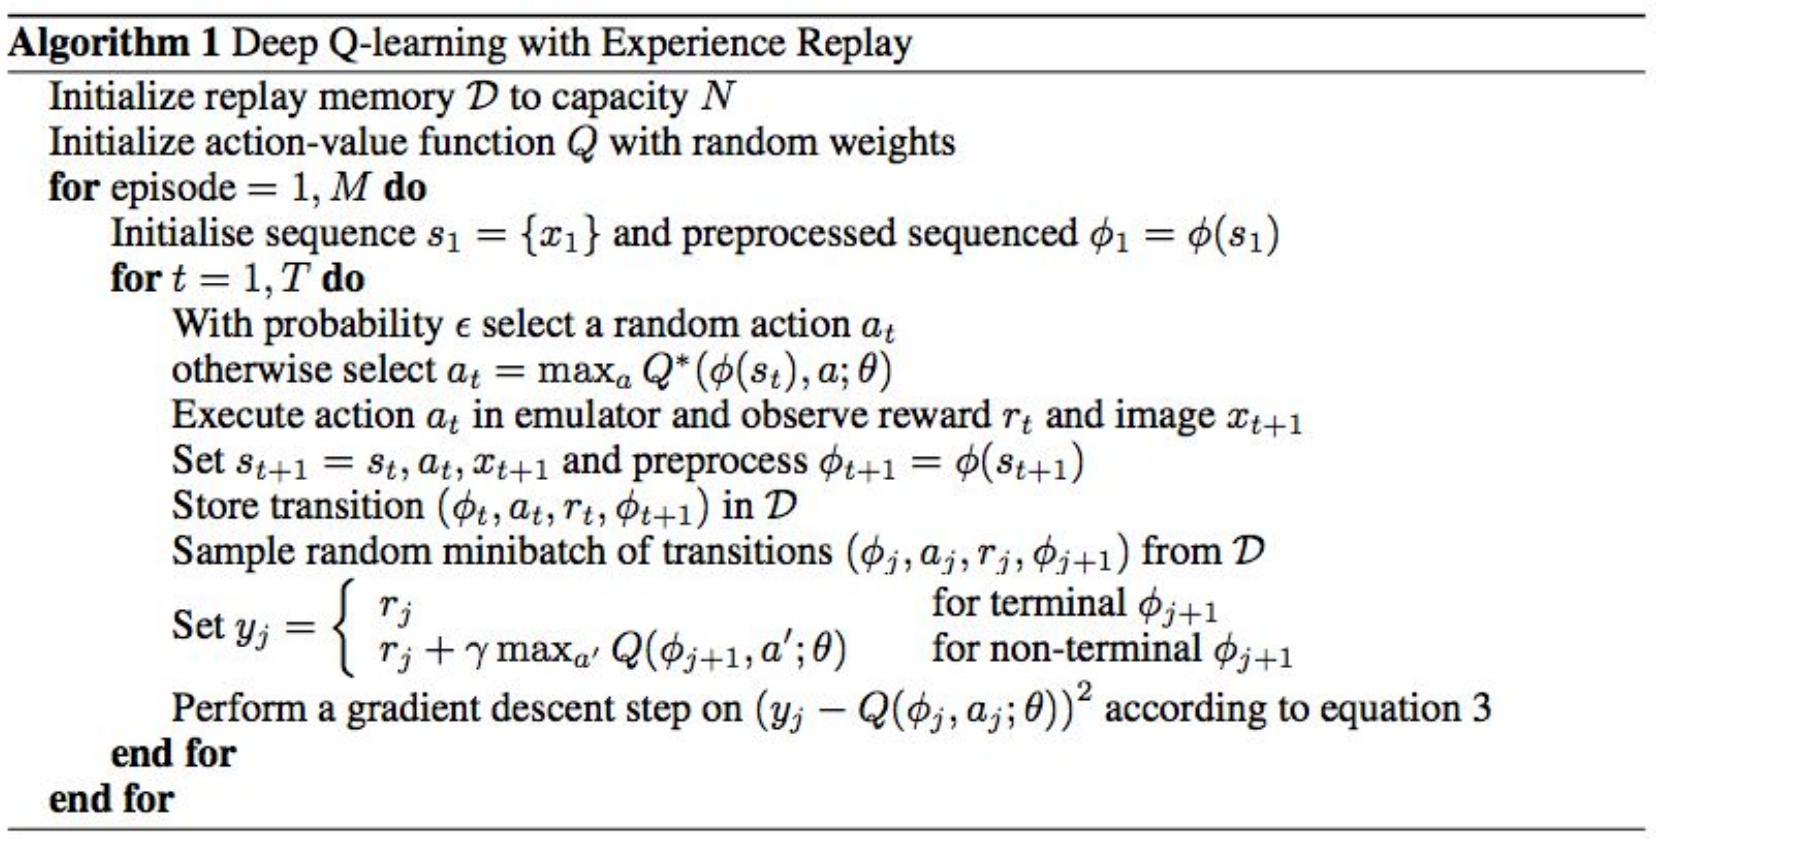
\includegraphics[width=0.9\textwidth,height=0.9\textheight,keepaspectratio]{images/dqn+sarsa/dqn.png}
    \end{figure}
\end{frame}

\begin{frame}{DQN with Target Network}
    \begin{itemize}
        \item DQN, as stated above, will have learning problems because the target and the prediction are not independant as they both rely on the same network.
        \item It's like a dog chasing it's own tail.
        \pause
        \item \textbf{Solution:} Use two separate $Q$-value estimators, each of which is used to update the other.
        \item The target values are calculated using a target Q-network. The target Q-network's parameters are updated to the current networks every $C$ time steps.
        \item Target network prevents the network from spiraling around.
    \end{itemize}
\end{frame}

\begin{frame}{DQN with Target Network Algorithm}
    \begin{figure}
        \centering
        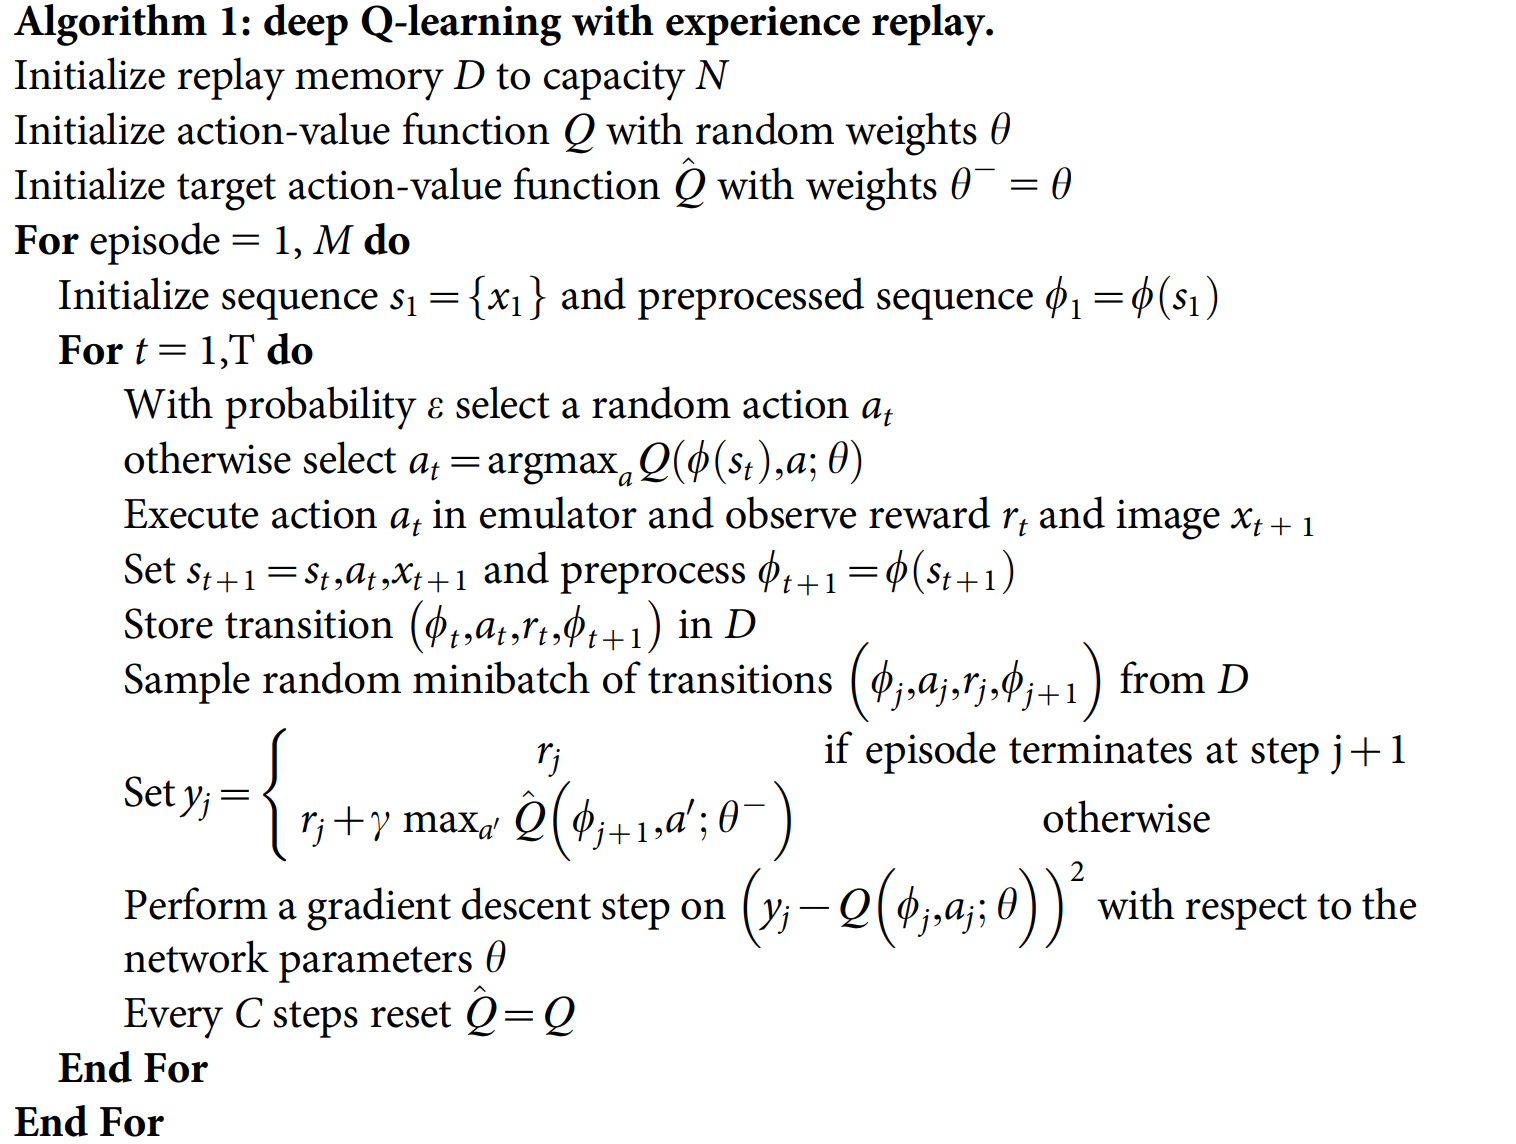
\includegraphics[width=0.9\textwidth,height=0.9\textheight,keepaspectratio]{images/dqn+sarsa/dqn_target.png}
    \end{figure}
    \footnotetext{Minh et al. https://www.nature.com/articles/nature14236}
\end{frame}